\documentclass{article}

\usepackage{amsmath, parskip, tikz}
\usetikzlibrary{automata}
\usetikzlibrary{positioning}
\usetikzlibrary{arrows}
\usepackage[margin=1.25in]{geometry}
\usepackage[shortlabels]{enumitem}

\renewcommand{\thesection}{\arabic{section}.}
\renewcommand{\thesubsection}{\alph{section}.}

\tikzset{
    node distance=2.5cm,
    every state/.append style={
        semithick,
        fill=gray!10
    },
    initial/.append style={
        initial text={},
        initial distance=0.5cm
    },
    accepting/.append style={
        double=gray!10,
        double distance=2pt,
        outer sep=1pt
    },
    every edge/.append style={
        draw,
        ->,>=stealth',
        auto,
        semithick
    }
}

\title{Homework 3: Regular Expressions and Non-Regular Languages}
\author{Will Griffin}

\begin{document}
    \maketitle

    \section{Regular Expressions vs Unix Regular Expressions} 
        \begin{enumerate}[(a)]
            \item Unix regular expressions have \textit{quantifiers}: if $\alpha$ is a regular expression, $a^{\{m, n\}}$ is a regular expression that matches at least $m$ and no more than $n$ strings that match $\alpha$. More formally, it matches all strings $w^{(1)} \cdots w^{(l)}$ where $m \le l \le n$, and for all such $i$ such that $1 \le i \le l$, $w^{(i)}$ matches $\alpha$. Prove that for any regular expression with quantifiers, there is an equivalent regular expression without quantifiers.

                A regular expression with a quantifier is written as such: $a^{\{m, n\}}$. To write this without quantifiers, we must understand that a quantifier $\{m, n\}$ on a regular expression matches the preceeding expression $i$ times, where $m \le i \le n$.

                There are three cases for this expression: 

                Case 1 ($m = n = 0$): $\alpha^{\{0, 0\}}$ means that $\alpha$ will be matched both at least and at most 0 times (or 0 times total), which means that this regular expression only matches the empty string. Therefore, $\alpha^{\{0, 0\}}$ can be written as $\varepsilon$.

                Case 2 ($m = 0, n > 0$): $\alpha^{\{0, n\}}$ means that $\alpha$ will be matched at least 0 times and at most $n$ times. Since any string $w$ can be written concatenated with the empty string (since $w = w \varepsilon = \varepsilon w$), the original regular expression can be written as $(\alpha \cup \varepsilon)^n$, as that will match either the expression $\alpha$ or the empty string $\varepsilon$ $n$ times.

                Case 3 ($0 < m \le n$): $\alpha^{\{m, n\}}$ means that $\alpha$ will be matched at least $m$ times and at most $n$ times. This can be broken up into two sections: matching $\alpha$ at least $m$ times and matching the potential additional $n-m$ times. Matching $\alpha$ at least $m$ times can be written as $\alpha^m$, and matching the potential additional $n-m$ times can be written as $(\alpha \cup \varepsilon)^{n-m}$. Concatenating these regular expressions together gives us the original regular expression without a quantifier: $\alpha^m (\alpha \cup \varepsilon)^{n-m}$.

                Therefore, any regular expression with a quantifier can be rewritten without a quantifier.

            \item Unix regular expressions have \textit{backreferences}. Give an example of a Unix regular expression that uses backreferences to describe a non-regular language, and prove that this language is not regular. Please write a full proof.

                Unix regular expression: ([0-1]*)\textbackslash1

                This can be written as the non-regular language $L = \{ww \mid w \in \{\texttt{0}, \texttt{1}\}\}$. To prove this language is non-regular, assume for the sake of contradiction the language is regular. Let $p$ be the pumping length given by the pumping lemma. Let a string $s = \texttt{0}^p \texttt{10}^p \texttt{1}$. Since $s \in L$ and $|s| > p$, the pumping lemma lets $s$ be written as $s = xyz$, where $y \neq \varepsilon$ and $|xy| \le p$. Then, because $|xy| \le p$, $y$ only contains \texttt{0}s. Let another string $s' = xyyz$. Since $|xy| \le p$ and $y$ only contains \texttt{0}s, $z = \texttt{0}^{p-k}\texttt{10}^p\texttt{1}$, where $|xy| = k$. Since we concatenate another $y$ in $s'$ compared to $s$, the first grouping of \texttt{0}s has more \texttt{0}s than the second grouping. Therefore, this string cannot be perfectly split in half, where the two substrings are equal. Therefore, $s' \notin L$. But, this contradicts the pumping lemma, where $s' \in L$. By proof of contradtiction, $L$ is non-regular.

        \end{enumerate}

    \section{Binary Addition}
        \begin{enumerate}[(a)]
            \item Show that the following is regular by writing an NFA for it:

                \begin{equation*}
                    B = \{w \in \Sigma^*_3 \mid \text{the bottom row of } w \text{ is the sum of the top two rows}\}
                \end{equation*}

                \begin{center}
                    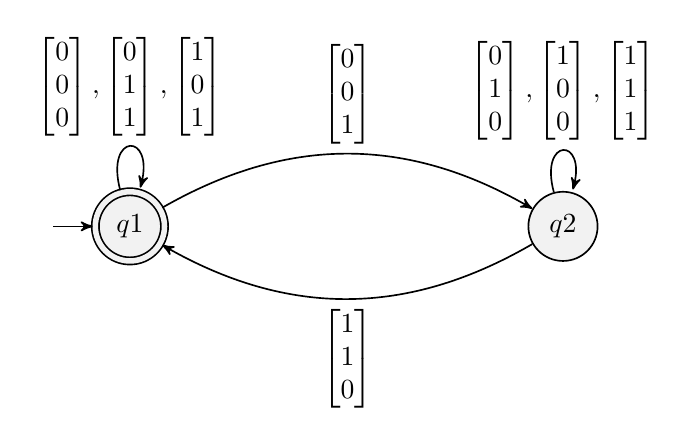
\begin{tikzpicture}
                        \node[state, initial, accepting] (q1) {$q1$};
                        \node[state, right of = q1, xshift=3cm] (q2) {$q2$};

                        \draw (q1) edge[loop above] node {$\begin{bmatrix}0 \\ 0 \\ 0\end{bmatrix}, \begin{bmatrix}0 \\ 1 \\ 1\end{bmatrix}, \begin{bmatrix}1 \\ 0 \\ 1\end{bmatrix}$} (q1)
                            edge[bend left] node {$\begin{bmatrix}0 \\ 0 \\ 1\end{bmatrix}$} (q2);
                        \draw (q2) edge[loop above] node {$\begin{bmatrix}0 \\ 1 \\ 0\end{bmatrix}, \begin{bmatrix}1 \\ 0 \\ 0\end{bmatrix}, \begin{bmatrix}1 \\ 1 \\ 1\end{bmatrix}$} (q2)
                            edge[bend left] node {$\begin{bmatrix}1 \\ 1 \\ 0\end{bmatrix}$} (q1);
                    \end{tikzpicture}
                \end{center}

            \item Let $\Sigma = \{\texttt{0}, \texttt{1}, +, =\}$, and prove that the following is not regular:

                \begin{equation*}
                    ADD = \{x = y + z \mid x, y, z \in \{\texttt{0}, \texttt{1}\}^* \text{ and } x = y + z \text{ is true}\}
                \end{equation*}

                I will prove that $ADD$ is not regular by proof by contradiction. Suppose $ADD$ is regular. The pumping lemma states that all regular languages have a pumping length $p$.

                Let a string $s = \texttt{1}^p = \texttt{0} + \texttt{1}^p$. The pumping lemma states that $s$ can be written as $s = xyz$, where $|y| > 0$ and $|xy| \le p$.  The lemma also states that any string $s' = xy^i z \in ADD$ for any $i \ge 0$. Since $|xy| \le p$, $y$ contains only \texttt{1}s.

                Let a new string $s' = xz$, that is, the case where $i = 0$. This string can be also written as $\texttt{1}^{p-k} = \texttt{0} + \texttt{1}^p$, where $k = |y|$. However, for this to be recognized by $ADD$, the equation must be true, and since the \texttt{1} terms on each side of the equation are not equal, this equation is clearly not true. Therefore, $s' \notin ADD$. 

                However, this contradicts the pumping lemma, which states that any $xy^iz \in ADD$ for any $i \ge 0$. Therefore, $ADD$ is not a regular language by proof of contradiction.

        \end{enumerate}

    \section{Similar But Different}
        \begin{enumerate}[(a)]
            \item Let $B = \{1^k w \mid w \in \{0, 1\}^*$ and $w$ contains at least $k$ \texttt{1}s, for $k \ge 1\}$. Show that $B$ is a regular language.

                From this language, we get the pattern that every string in $B$ must start with a $1$ and contain at least 1 other 1 in the string. This can be written using the following regular expression:

                \begin{equation*}
                    1(0 \cup 1)^*1(0 \cup 1)^*
                \end{equation*}

                This regular expression accepts any number of $1$s followed by any number of $0$s followed by at least one $1$, followed by any number of $0$s or $1$s. This expression accepts all $1^k w$ where $w$ contains at least $k$ $1$s. Since the minimum requirement of $k = 1$ is met by any string accepted by that regular expression, the language $B$ is regular. 

            \item Let $C = \{1^k w \mid w \in \{0, 1\}^*$ and $w$ contains at most $k$ \texttt{1}s, for $k \ge 1\}$. Prove that $C$ is not a regular language.

                Assume for the sake of contradiction that $C$ is a regular language. Therefore, by the pumping lemma, we get a certain pumping length $p$. 

                Let a string $s = 1^p 1^p$. Since $s \in C$, by the pumping lemma, $s$ can be written as $s = xyz$, where $|y| > 0$, $|xy| \le p$, and $xy^iz \in C$ for all $i > 0$. 

                Let another string $s' = xz$, the case where $i = 0$. Since $|xy| \le p$, $xy$ must consist of $1$s entirely from the first substring of $1$s. Therefore, $s'$ can also be written as $s' = 1^{p-j} 1^p$, where $j = |y|$. Since $p-j < p$, $s' \notin C$. This contradicts the pumping lemma, which stated that $s' \in C$. 

                By contradiction, $C$ is not a regular language.
                
        \end{enumerate}

    
\end{document}
